\documentclass[conference]{IEEEtran}

\usepackage{cite}
\usepackage[pdftex]{graphicx}
\graphicspath{{./figures/}}
\usepackage[cmex10]{amsmath}
\usepackage{array}
\usepackage{siunitx}
\sisetup{detect-all} % use text font instead of math font

% correct bad hyphenation here
\hyphenation{op-tical net-works semi-conduc-tor}

\begin{document}
\title{Near-Threshold Computing Revisited}

\author{\IEEEauthorblockN{Chris Gonzales\\ Mario Lok\\ Judson Porter}}
%\IEEEauthorblockA{School of Electrical and\\Computer Engineering\\
%Georgia Institute of Technology\\
%Atlanta, Georgia 30332--0250\\
%Email: http://www.michaelshell.org/contact.html}
%\and
%\IEEEauthorblockN{Homer Simpson}
%%\IEEEauthorblockA{Twentieth Century Fox\\
%%Springfield, USA\\
%%Email: homer@thesimpsons.com}
%\and
%\IEEEauthorblockN{James Kirk\\ and Montgomery Scott}
%\IEEEauthorblockA{Starfleet Academy\\
%San Francisco, California 96678-2391\\
%Telephone: (800) 555--1212\\
%Fax: (888) 555--1212}}

% make the title area
\maketitle


\begin{abstract}
%\boldmath
The abstract goes here.
\end{abstract}

\section{Introduction}
\label{sec:intro}

Power consumption and heat removal have become two of the top concerns in the datacenter space\cite{EPA_2007}. 
According to the International Technology Roadmap for Semiconductors, power consumption for each generation of chips is growing, making it one of the most significant roadblocks to future scaling \cite{Devised_2009}. 

One recently proposed  solution to this increased power is to operate the microprocessor at a significantly lowered voltage, approaching the transistor threshold voltage~\cite{Dreslinski:2010ez}. 
This near-threshold computing~(NTC) will yield approximately a 10x energy savings at the cost of 10x performance loss and a 20x total performance uncertainty. 
The NTC proposal claimed that many of these downsides can be mitigated by techniques such as device optimizations, variation tolerant circuit design, and body biasing as well as architectural changes such as increased parallelism and a move to a clustering-based architecture.

We have shown that many of the ideas presented in Dreslinski's NTC paper \cite{Dreslinski:2010ez} are ineffective at recovering the performance lost due to near-threshold computing, especially in the context of a datacenter environment. 
Although datacenters have a strong motivation to reduce their power consumption, the performance sacrifices inherent to NTC makes it an impractical choice for future servers.

In Section~\ref{sec:deltavth}, we will introduce an expression for the dependency of delay on operating voltage in near-threshold, showing that small variations in supply or threshold voltages can lead to large differences in performance.
%Section~\ref{sec:deviceoptimization} will expand upon this to show that the potential device optimizations cited by Dreslinski's NTC paper as methods to increase transistor speed will be ineffective in the near-threshold regime.
Expanding on these concerns over variability, Section~\ref{sec:criticalpaths} derives a conservative model for how the number of potential critical paths increases due to the additional delay variation inherent in near-threshold computing and Section~\ref{sec:softedge} raises concerns about the ability of soft-edge flip flops to overcome delay variations in near-threshold designs.
Section~\ref{sec:regulators} discusses power delivery concerns, both in terms of supply noise and regulator inefficiency. 
Concerns about the methodology of Dreslinski's proposed clustering architecture are addressed in Section~\ref{sec:clustering}, which is generalized in Section~\ref{sec:darksilicon} to show that any parallel architecture will have problems regaining performance lost to NTC.


\section{Determining the effect of $\Delta V_{th}$}
\label{sec:deltavth}

\begin{figure}[thpb]
    \centering
    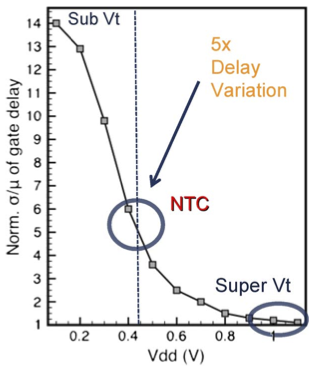
\includegraphics[width=0.4\textwidth]{dreslinski_voltage_delay}
    \caption{Dependence of delay on voltage in near-threshold.~\cite{Dreslinski:2010ez}}
    \label{fig:voltage_delay}
\end{figure}
Because the delay of a gate has a strong dependence on gate voltage in near-threshold operation (see Figure~\ref{fig:voltage_delay}), determining the effect of small changes in $\Delta V_{th}$ is essential to understanding the operation of near-threshold circuits.
This delay is determined by the drain current of the transistor.
The drain current has fundamentally different relationships to voltage in sub- and super-threshold operation; in the sub-threshold mode, the current has an exponential relationship to voltage~\cite{Enz:1995vs} 

\begin{equation}
I_D \propto e^\frac{V_P-V_S}{U_T}
\end{equation}

while super-threshold operation yields a quadratic relationship

\begin{equation}
I_D \propto (V_P-V_S)^2
\end{equation}

where $V_P=V_G-V_{TH}-V_\gamma$ with $V_\gamma$ being a function of body effect.

For near-threshold operation, however, an interpolation has to be used to bridge these two expressions~\cite{Enz:1995vs}, giving us the forward drain current as

\begin{equation}
\label{eqn:nth_current}
I_D \propto \left[\ln\left(1+e^\frac{V_G-V_{TH}-V_\gamma}{2}\right)\right]^2
\end{equation}

The relationship between delay and current, as derived in~\cite{Hanson:2007uu}, is
\begin{equation}
\label{eqn:delay}
t_p = \frac{k_d\cdot C_L\cdot V_D}{I_{on}}
\end{equation}

When Equation~\ref{eqn:nth_current} is combined with Equation~\ref{eqn:delay}, the expression for delay becomes

\begin{equation}
\label{eqn:nth_delay}
t_p\propto\frac{V_D}{\left[\ln\left(1+e^\frac{V_G-V_{TH}-V_\gamma}{2}\right)\right]^2}
\end{equation}
 
 showing that variations in $V_G$ or $V_\gamma$ that are considered insignificant in super-threshold operation can cause large differences in transistor delay.
For example, a 50mV difference in threshold voltage could result in a $7.5\%$ reduction in FMAX and a 50mV difference in $V_G$ can result in a $11\%$ reduction in FMAX; the same difference in $V_G$ at super-threshold results in a $0.7\%$ reduction.

In near-threshold operation even very small differences in voltages and device characteristics, those of a magnitude that can easily be overlooked in super-threshold operation, have a dramatic effect on transistor operating frequency. 
This means that not only does near-threshold operation translate to a slower device, but it also translates to a much more variable device.
Looking at near-threshold as having 10x lower performance is not enough; one must also consider the additional safety factor needed to account for this variation.

\section{Device Optimizations}
\label{sec:deviceoptimization}

Dreslinski et al. \cite{Dreslinski:2010ez} suggest modifications of the transistor structure to reduce delay by reducing inverse sub-threshold slope ($S_S$). 
This can take the form of either modifying the channel doping profile \cite{Paul:2004cx} or increasing oxide length \cite{Hanson:2007uu}.

Hanson shows that the main delay benefit from scaling $S_S$ comes from the assumption that the system voltage set to the minimum energy point of the CMOS logic, a point far into sub-threshold that is proportional to $S_S$~\cite{Hanson:2007uu}. 

\begin{align}
t_p&=\frac{k_d \cdot C_L \cdot K_{V_{min}} \cdot S_S}{I_{off} \cdot 10^\frac{K_{V_{min}S_S}}{S_S}}\\
&\propto \frac{C_L \cdot S_S}{I_{off}}
\end{align}

For near-threshold operation, the voltage is instead set by the transistor threshold voltage. 
With the voltage dependence on $S_S$ removed, this equation instead becomes

\begin{equation}
t_p \propto \frac{1}{e^\frac{V_{D}-V_{TH}}{S_S}}
\end{equation} 

which is a much weaker effect considering that $S_S$ in the range of 80-90mV/decade. 

The actual correlation of delay to $S_S$ is even weaker because Hanson is using an equation that assumes the circuit is operating far sub-threshold. 
As $V_{DD}$ passes $V_{TH}$, the current and delay begin to instead scale with an interpolation between super-threshold and sub-threshold models rather than just the sub-threshold model. 
Because the super-threshold model doesn't have a reliance on $S_S$, this means that the effect of modifications to $S_S$ on system delay get weaker as voltage moves from sub-threshold into the near-threshold regime.

 Raychowdhury \cite{Raychowdhury:2006fu} shows this weakening of $S_S$'s effect on delay in Figure~\ref{fig:doping}. As $V_DD$ increases, the delays of the standard and optimized CMOS devices get closer.
  
\begin{figure}[thpb]
    \centering
    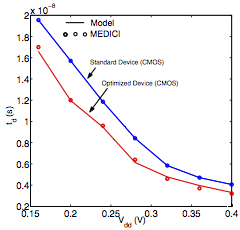
\includegraphics[width=0.4\textwidth]{raychowdhury_doping.png}
    \caption{Effect of sub threshold slope optimization on delay at different voltages.~\cite{Raychowdhury:2006fu}}
    \label{fig:doping}
\end{figure}
 
Although Dreslinski is correct that several research groups have shown optimizations that allow sub-threshold devices to operate at a reduced delay\cite{Dreslinski:2010ez}, citing these as evidence that near-threshold delay can also be improved is misleading. Near-threshold devices, by their very definition, operate in a different region of the transistor's current-voltage curve and optimizations for sub-threshold operation will have a greatly diminished effect on near-threshold delays.
\section{Increase in the number of critical paths}
\label{sec:criticalpaths}

The increased variance in delay caused by near-threshold operation is directly responsible for an increase in the number of critical paths.
A critical path can be defined as any path that has a high probability of exceeding a given clock \cite{Wang:2004bw}.
For our cases of trying to find the maximum frequency a given device can run, we can instead consider a critical path as a path that has a high probability of setting FMAX; that is, of being the longest path in the system.
  
Consider a distribution of nominal delays of paths within a chip (Figure~\ref{fig:normal}).
In the case of no variations, clock speed is set by the path with the highest nominal delay.
Once delay variation is added in, however, points that are close in delay to the path with the highest nominal delay could act instead as the critical path in a portion of chips.
This means that it is any path that falls within $n\frac{\sigma_v}{\mu}$ of the maximum nominal delay for a given n where $\sigma_v$ is the standard deviation of the timing path variation distribution.
 
\begin{figure}[thpb]
    \centering
    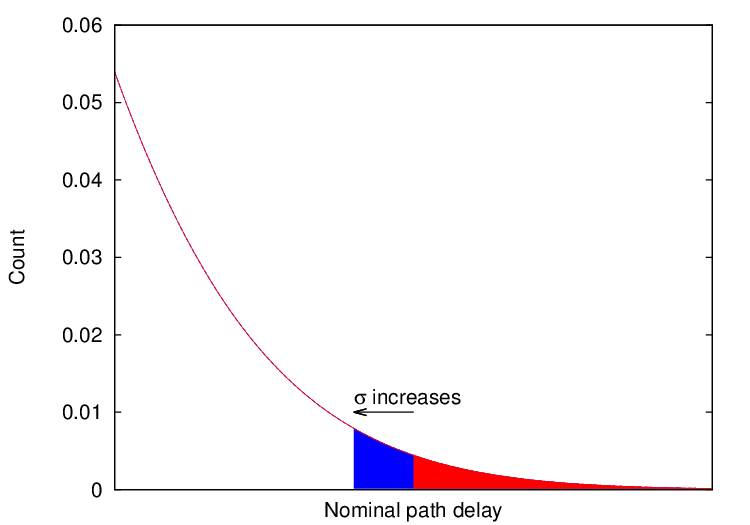
\includegraphics[width=0.4\textwidth]{normal.png}
    \caption{As $\sigma_v$ increases, the number of critical paths increases}
    \label{fig:normal}
\end{figure}
 
 Although the shape of the nominal delay distribution will vary depending on the design of the chip, if it is assumed this shape is strictly convex, the number of critical paths $N_{cp}$ increases at least linearly with $\sigma_v$.
Considering that $\frac{\sigma_v}{\mu}$ increases approximately 7x as the voltage drops into the near-threshold regime, there is at least a 7x increase in the number of critical paths.
This will translate into a reduction in the maximum frequency of the design\cite{Bowman:2002cp} and added design complexity, as more critical paths will have to be optimized.


 \section{Soft-edge clocking}
Another proposal has been the use of soft-edge clocking to increase speed in near-threshold devices by reducing the dependence on critical path delay \cite{Wieckowski:2008bo}.
 In this design, a traditional D-flip flop is modified to be driven by two offset clocks, generating a short transparency window.

The clock delay generation becomes an issue as variability increases.
 The simple method used in the paper of having a chain of inverters would be heavily susceptible to process variations.
 As the two clocks move closer to each other, the soft-edge effect becomes minimized; as the two clocks drift further apart, race-through becomes a concern.
 The frequency improvement of the SFF design over a standard DFF relies heavily on the size of this softness window, as shown in figure **INSERT FIGURE NUMBER**, but as $\sigma_v/\mu$ increases, the variance of the delay through this clock delay system also increases and the target transparency window of the flip flop gets driven more by the need to keep the SFF operating in the permitted region rather than the ideal softness window.

**INSERT FIGURE 13 FROM HANSON**

\section{Voltage Regulators}

We already know logic gates computes more efficiently at a supply voltage level
that is near the device threshold voltage. When we attempt to translate the
energy efficiency of these gates to the energy efficiency of a whole system, we
need to carefully evaluate the associated overhead.
Both~\cite{ISLPED:2011}
and~\cite{Pitfall:2010} raised the concern that the efficiency
of the voltage regulator would be lower for delivering power to a near-threshold
computing design. \cite{ISLPED:2011} presents evidence that
typical voltage regulator efficiency is lower at light load and argues that if a
near threshold design consumes less power the efficiency will be lower.
\cite{Pitfall:2010} considers the case where the chip supply
voltage is generated with an on-chip switch-capacitor converter. They shows that
the efficiency of the regulator is at 90\% for an output voltage of 1.2V and is
at 70\% for an output voltage of 0.5V.

In the context of server computing, the power is delivered to the
microprocessors typically through a buck converter which down converts the 12V
mother board voltage~\cite{Server:2006}. Although it is
difficult to derive a quantitative comparison between the efficiency of a 1.2V
output for an above threshold design and a 0.5 output for a near threshold
design, it is possible to consider the difference in requirement for these two
regulators and understand where the difference in efficiency may come in. 

The performance of digital circuits is highly susceptible to power supply noise.
This susceptible is worse when the design is operating in the near threshold
region, as shown earlier in figure ~\ref{fig:voltage_delay}). On the other hand,
the power supply noise is a function of load stepping and decoupling capacitor.
Since load stepping is a function of the processor architecture, we can assume
simply scale down the supply voltage would not change the magnitude of the power
supply noise. This power supply noise is a larger percentage of the supply
voltage when the design is operating in near threshold region. As a result, it
cause more delay variation in the design. As performance variation has already
been one of the key limiting factors for near threshold computing, it become
necessary to suppress this voltage noise at the price of efficiency, board area
or chip area by increasing the feedback loop bandwidth and adding more
decoupling capacitors.

In addition,  one of the goals of employing near threshold computing for servers
is to reduce power consumption while maintaining throughput. However, unless
near threshold computing can achieve processor power reduction by a factor that
is larger than the factor supply voltage is reduced by, the current drawn by a
near threshold design is going to be higher. This higher output current is
particular problematic for the power loss due to the output rectification. The
efficiency loss in the output rectification is the ratio between the output
voltage and the voltage drop across the output transistor. Since the output
voltage is small, the regulator is more sensitive to voltage drop across the
output transistor. On top of that, the higher output current further increases
the voltage drop across the output stage.  


\section{Body Biasing}
\label{sec:bodybiasing}

Bodying biasing has been proven to be effective in compensating for the
performance loss of a design due to within-die systematic variation and
intra-die variation. However, it has been increasingly challenging to employ
this technique because the effect of body biasing is decreasing as transistor
technology scales to smaller dimension. In every technology generation, the gate
oxide capacitance $C_{ox}$ is scaled up for a factor 0.7 and the doping
concentration of the channel is scaled up by a factor of 0.7. By equation X1,
the combined effect of scaling these two parameters reduces the body effect
parameter gamma, which determines the effectiveness in using body biasing to
modify the device threshold voltage as shown in equation X2.

\begin{equation}
V_{T} = V_{TO} + \gamma ( \sqrt{ | {V_{SB} + 2\phi_{F} | } } - \sqrt{ | 2\phi_{F} | } 
\end{equation}

\begin{equation}
\gamma = (1/C_{ox})\sqrt{2q\epsilon_{si}N_A}
\end{equation}

With various resolution enhancement technique, the systematic variation in gate length has been kept to a steady percentage of the gate length variation in recent technology node~cit{Intel:2009}. Intel shows that sigma of the system variation gate length variation is managed to apprximately 3% across different technology node~cite{Intel:2009}. However, due to the inherent resolution limitation in current lithogothy process, percentage of gate length variation in future technology generation may start to increase again~cite{OPC20}.    


Under these two trends, the need for body biasing compensation is potentially increasing
while the effectiveness of body biasing is decreasing. Nevertheless, when the
body biasing technique is applied to a near threshold design, the delay tuning
range is much larger for the same amount of threshold modulation. Yet at the
same time, since a near-threshold design is more sensitive to process variation,
it is not obvious whether body biasing is more effective for a near threshold
design. 

To make a quantative comparison between the effectiveness of body biasing for both an
above threshold design and a near threshold design across different technology
nodes,  we simulate the propagation  delay of a 6 FO4 inverter delay chain in
32nm, 22nm and 16nm using ASU Technology Predictive Model \cite{PredictiveModel}. To simplify the
analysis, the only variation considered is within-die systematic variation. To limit the leakage power overhead to 100\% when body biasing is applied, the maxiumum forward body biasing is set to be 0.2V.  Table~\ref{body1} and table~\ref{body2} shows the delay of the inverter chain for zero body biasing and maxiumum forward body biasing when no variation is presented. The results show that body biasing indeed influence the delay of the inverter chain by a large percentage in the near threshold region, but across technolgoy node, the performance improvment with maxiumum body biasing is decreasing.   


\begin{table}
  \caption {Peformance improvement by body-biasing in above threshold computing} 
  \centering 
  \label {body1}
  \begin{tabular}{ | l | l | l | l | }
    \hline
    & 32nm & 22nm & 16nm \\ \hline
    nominal delay(ps) & 45.0 & 26.0 & 17.2 \\ \hline
    maxiumum $V_{BBfwd}$ (ps)  & 41.3 & 24 & 15.9 \\  \hline
    percentage change  & 8.2\% & 7.7\% & 7.5\% \\ 
    \hline
  \end{tabular}
\end{table}



\begin{table}
  \caption {Peformance improvement by body-biasing in near threshold computing}  
  \centering
  \label {body2}
  \begin{tabular}{ | l | l | l | l | }
    \hline
    & 32nm & 22nm & 16nm \\ \hline
    nominal delay(ps) & 1709 & 464 & 207 \\ \hline
    maxiumum $V_{BBfwd}$ (ps)  & 889 & 278 & 139 \\  \hline
    percentage change  & 48\% & 40\% & 33\% \\ 
    \hline
  \end{tabular}
\end{table}

Table~\ref{compensation} shows the result when variation is included in the model. The effectiveness of process compensation by body biasing is measured in terms of magnitude of gate length variation body biasing can restore. As suggestied by the model, although the compensation is very effective in 35nm for near threshold computing, being able to compensate for 21.25\% of gate length variation, this number will quickly be quickly be reduced to 5.6\% in two technolgoy node. As the sigma of systematic variation in gate length is approximately 3%, body biasing can only correct for 2 $\sigma$ in two generations. Thus, in future technology generation, the body biasing technique would not be sufficient to offset the delay variation for near threshold computing.    

\begin{table}
  \caption {Variation compensation by body-biasing}  
  \centering
  \label {compensation}
  \begin{tabular}{ | l | l | l | l | }
    \hline
    & 32nm & 22nm & 16nm \\ \hline
    above Vt(nm) & 1.2 & 0.8 & 0.3 \\ \hline
    \% compnesation in L  & 3.75\% & 3.6\% & 1.9\% \\ \hline
    near Vt(nm)  & 6.8 & 1.9 & 0.9\\  \hline
    \% compnesation in L & 21.25\% & 8.64\% & 5.62\% \\ 
    \hline
  \end{tabular}
\end{table}


\section{Near-Threshold Parallel Architectures} \label{sec:clustering}

Deslinkski et al.~\cite{dreslinski2010near} claim ``In applications where there
is an abundance of thread-level parallelism the intention is to use 10 s to 100
s of NTC processor cores that will regain 10-–50X of the performance, while
remaining energy efficient.'' In order to regain the performance lost from using
near-threshold techniques, Zhai et al.~\cite{Zhai:2007kn} and Dreslinski et
al.~\cite{Dreslinski:2007id} present a technique for leveraging parallelism in
the NTC regime. The proposed architecture groups multiple slower-cores into
clusters which share a faster L1 cache. The cache operates at $n$ times higher
frequency than the cores, where $n$ is the number of cores in a cluster. This is
motivated by the observation that SRAM has a higher energy optimal $V_{dd}$ and
$V_{th}$ than logic due to its lower activity factor and higher leakage energy
component. As a result of SRAMs higher energy optimal $V_{dd}$, the energy
optimal frequency of memory is higher than that of logic.  Based on this
observation, the proposed technique shares the first-level cache with multiple,
slower cores allowing individual tuning of $V_{dd}$ and $V_{th}$ between the
cores and memory. Using this architecture, the cores still maintain single-cycle
memory accesses while the core and memory can each operate at their energy
optimal $V_{dd}$ and $V_{th}$. Running the memory at a higher $V_{dd}$ also help
mitigate many of the reliability issues affecting SRAM in the near-threshold
regime.

Using this technique, a 71\% energy savings over a baseline single core machine
on the highly parallel SPLASH2 benchmark is demonstrated. However, in
investigating these claims, some shortcomings with this approach are revealed.
Of primary concern is the large area overhead required to achieve the same
benchmark performance. In order to achieve the same performance as a single core
baseline system, 6 cores and 3 times the baseline amount of cache were required.
It is important to remember that these results are being presented in comparison
to a single core reference on a highly parallel workload. By Amdahl's law, the
speedup from parallelism will have diminishing returns as more cores are added.
The corollary is that the biggest benefit from parallelism will be realized by
going from a single core to several cores.  It would require a larger number of
cores to achieve the same level of parallelism when comparing with a baseline
system that included more than a single core. In fact, to achieve the same
performance as the baseline, some benchmarks require as many as 16 cores and 32
times as much L1 cache (\SI{2}{\mega\byte} vs \SI{64}{\kilo\byte}). Their
results show very little energy efficiency improvement when moving from a
traditional $V_{dd}$ scaled CMP to a clustered architecture without $V_{th}$
tuning.

The clustering technique also uses separate $V_{th}$ tuning for the core and
cache to find the energy optimal voltage for the same performance. However, in
examining what these voltages actually are, it is revealed that neither $V_{dd}$
of the cache nor the logic is actually in the near-threshold regime as defined
by the paper, and both are in fact operating at a $V_{dd}$ 2x--3x higher than
the selected $V_{th}$. In modern process technologies, the standard is $V_{dd}$
already approaching 2x $V_{th}$. As described in Section~\ref{sec:bodybiasing},
the techniques for tuning $V_{th}$ are also becoming less effective.

One final concern is that while energy optimal cluster configurations are
presented for each SPLASH2 benchmark, no co-optimized configuration is given.
This could potentially be an issue as the energy optimal range of cores,
clusters, cache sizes, $V_{dd}$ and $V_{th}$ is large. It is unclear what the
energy savings across benchmarks for different configurations will be.

\section{Shortcomings of Application Parallelism} \label{sec:darksilicon}

Dreslinski et al.~\cite{Dreslinski:2010ez} state ``More gates can now fit on a die, but a growing fraction cannot actually be used due to strict power limits.''
This issue is commonly referred to as dark silicon.
While the number of transistors on a given die has been doubling every generation, the number of transistors that can be powered for a fixed power budget has not been increasing due to the slowing of transistor energy scaling.
Since power budgets have not been increasing, a situation has arisen where future generations of chips will potentially have more transistors than can be powered at any given time.

Dark silicon seemingly presents an opportunity for near-threshold computing, and as a way of addressing the large area overheads of the clustering architectures discussed in Section~\ref{sec:clustering}.
By reducing the power consumed per-core, more cores can be simultaneously powered.
Since these cores could not be powered in a super-threshold chip, this represents an opportunity for near-threshold chips to regain performance compared to super-threshold operation.

\begin{figure}[thpb] \centering
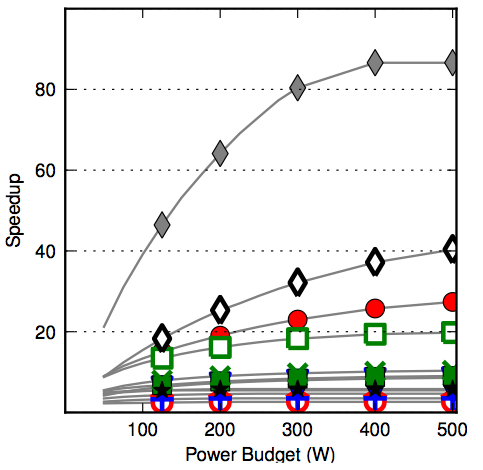
\includegraphics[width=0.3\textwidth]{esmaeilzadeh_power_speedups.png}
\caption{Projected speedups on PARSEC benchmarks while the chip power limit (and therefore the number of cores) is increased.~\cite{Esmaeilzadeh2011Dark-silicon-an}}
\label{fig:power_speedups}
\end{figure}

While dark silicon is an opportunity for devices to reach higher levels of integration, recent studies analyzing dark silicon have not borne out the promise of higher levels of performance with increasing core counts.
Esmaeilzadeh et. al~\cite{Esmaeilzadeh2011Dark-silicon-an} developed an analytical model analyzing the impact of dark silicon for a range of CMP configurations in future process technologies.
They show projected speedups for these configurations using the PARSEC benchmark suite, which represents workloads similar to the SPLASH2 benchmark suite used in clustering architecture discussed in Section~\ref{sec:clustering}, indicating that both works are targeting similar application spaces.
This analytical model does project that dark silicon will become a significant portion of CPU area in the near future, dominating as soon as 2016 with a conservative scaling model.
The authors also analyze the case where the power constraint is lifted, which allows more cores to be powered and reduces the amount of dark silicon.
Figure~\ref{fig:power_speedups} shows the projected speedups on different PARSEC benchmarks as the chip power is increased.
The paper projects that if the amount of parallelism in applications were increased to 99\%, then the best case speedup for power limited cores in \SI{8}{\nano\meter} is 15x relative to a quad-core Nehalem processor at \SI{45}{\nano\meter}.
However, 8 out of 12 PARSEC benchmarks achieve no more than 10x speedup with an unconstrained power budget, as shown in Figure~\ref{fig:power_speedups}. 
This indicates that the amount of parallelism in general-purpose parallel workloads will be exploitable even by future power constrained multi-core chips.
While near-threshold computing would allow more chips to be powered, it would not realize a significant speedup on most general-purpose parallel workloads due to the lack of exploitable parallelism.

\begin{figure}[thpb]
\centering
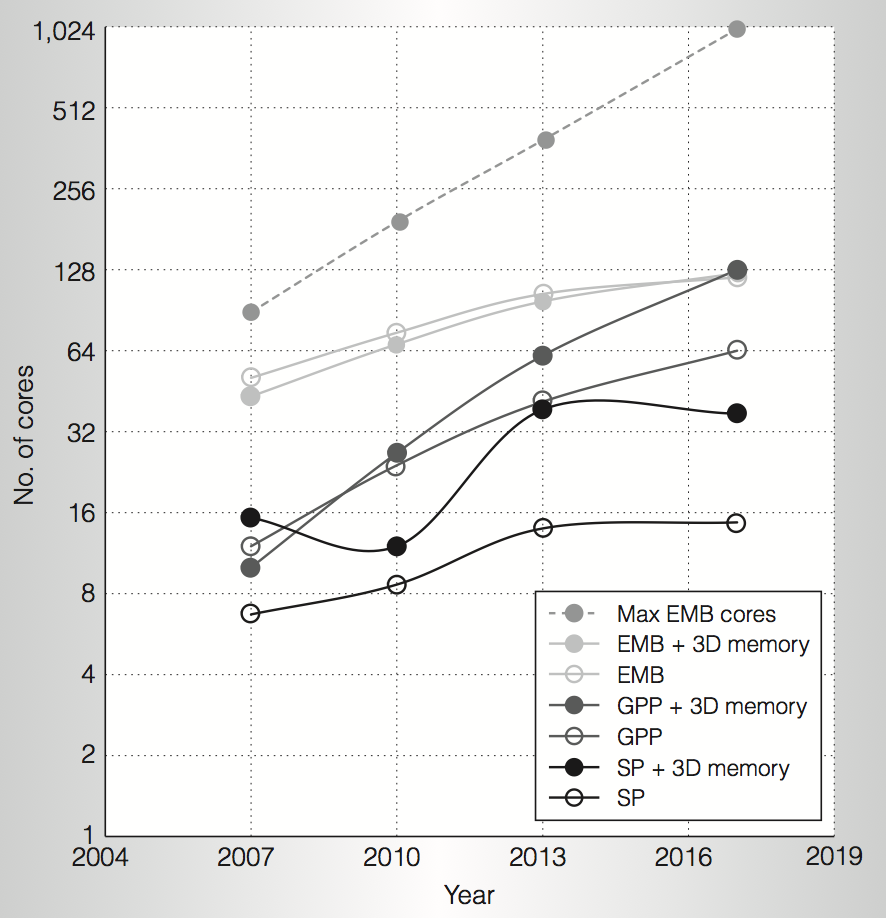
\includegraphics[width=0.4\textwidth]{hardavellas_core_counts.png}
\caption{Projections for core count scaling.~\cite{Hardavellas:2011de}}
\label{fig:core_counts}
\end{figure}

\begin{figure}[thpb]
\centering
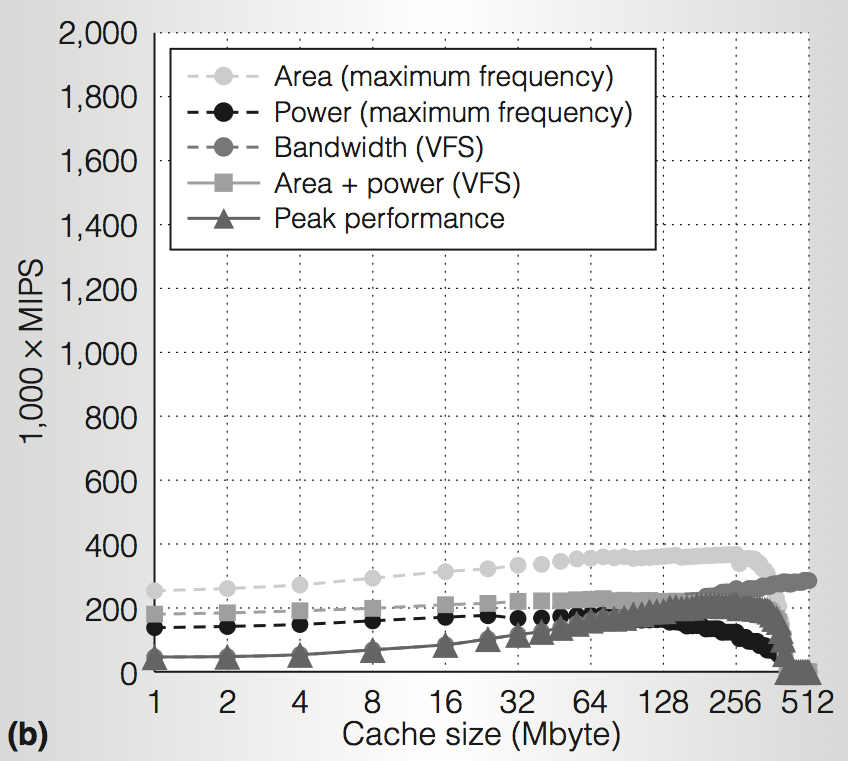
\includegraphics[width=0.4\textwidth]{hardavellas_emb_performance.png}
\caption{Embedded core scaling.~\cite{Hardavellas:2011de}}
\label{fig:emb_performance}
\end{figure}

Further work by Hardavellas et al.~\cite{Hardavellas:2011de} confirms the observation that future speedups are limited by application level parallelism, not power constraints.
In this study the authors built an analytical chip performance model for different types of cores, including low-power embedded cores (EMBs) similar to an ARM11 MPCore, and modeled how the performance of these chips scale in future process technologies given area, power, and memory bandwidth constraints.
Figure~\ref{fig:core_counts} shows projected core count scaling trends in future process technologies.
The difference between the ``Max EMB cores'' line and the ``EMB'' line represents the difference in how many cores can fit on a die versus how many can be powered given current chip power constraints.
Their model projects that in 2017 over 1024 cores will be able to fit on a die, but only 12\% of them will be able to be powered at any given time.
Again, this looks like an opportunity for near-threshold computing to increase core counts over traditional super-threshold CMPs.

Figure~\ref{fig:emb_performance} shows the maximum performance of an EMB-based CMP given different constraints for a 99\% parallel workload.
The ``Area (maximum frequency)'' line represents the best performance with only a die area constraint, while the ``Peak Performance'' line represents the best performance factoring in area, power, and memory bandwidth constraints.
While the constrained case only has 12\% of the cores of the area constrained case, it only has approximately half the performance of the unconstrained case.
Again, the performance is limited by the application parallelism, not the number of cores integrated onto the chip.

While NTC processors could support increased core counts over super-threshold chips, they would not be able to gain back a significant amount of the performance loss as super-threshold core counts are already approaching the limits of exploitable parallelism in general-purpose workloads.
Without a focus on increasing the amount of parallelism in these applications, opportunities for NTC processors to regain performance loss through parallelism will be limited.

\section{Conclusion}
\label{sec:conclusion}

In the general-purpose server computing space, near-threshold computing is not a viable solution to achieving more energy efficiency computing while maintaining system throughput.
The inherent problems of slower devices and increased variability in near-threshold computing are still major barriers for a near-threshold server processor to achieve the same throughput level as a super-threshold server processor.
The state-of-the-art device optimization for low voltage operation provides little performance boost to transistors operating in the near-threshold region.
Soft-edge clocking becomes less effective in combating variation in near-threshold.Adding to the difficulties of applying near-threshold computing, the inefficiency of delivering power to a low voltage chip and the stricter requirement on the power supply diminishes the power reduction benefits from operating the server processor at low voltage.
Worst of all, the marginal parallelism that can be extracted from the already highly parallel server workload is far from enough to bridge the 10X performance gap between near-threshold computing and traditional above threshold computing.


\bibliographystyle{IEEEtran}
\bibliography{IEEEabrv,bibtex,bibtex_chris}

\end{document}


